% !TEX root = 00_main.tex
% TLDR: Four results (exp 22, exp 25, earlier panel exp 67) and the pending judge-building experiment (exp 27).
\section{Experiments}
\label{sec:experiments}
Every number below is copied from the results file of its experiment, or recomputed from the anonymized data by a script named there (\cref{app:trace}); tables list RPS, CE and TVD first and correlations last.

\subsection{Does the selected judge beat the constant?}
\label{sec:exp22}
We re-score, on the full panel, the judge that had been selected for its correlations: GPT-6 Sol and Claude Opus 5.5 (H2 prompt, three calls each) on the old set, with the canonical $10/5/10$ task split.
The constant is the training-task rating distribution.
\Cref{tab:exp22} shows that correlation jumps between splits (Spearman $0.64$, $0.88$, $0.83$) while test RPS ($0.195$) is no better than the constant ($0.184$): the paired difference is $+0.012$ with interval $[-0.090,+0.109]$.
On the 24 ordinary test artifacts (two test tasks have placeholder references) the judge is nominally worse, RPS $0.223$ against $0.178$, and test Spearman falls from $0.83$ to $0.65$ with interval $[-0.17,+0.92]$.
Cross-entropy of the judge is far above the constant on every split, but it is floor-dependent (\cref{app:floor}); the judge's test TVD ($0.628$) is below the constant's ($0.665$), but the paired difference ($-0.037$, $[-0.209,+0.126]$) includes $0$.

\begin{table*}[t]
\caption{The selected judge (GPT-6 Sol and Claude Opus 5.5, H2 prompt, 6 calls) by split on the old set. RPS has the task-cluster bootstrap 95\% interval; the constant is the training-task distribution. RPS, CE and TVD first, correlations last.}
\label{tab:exp22}
\centering\small
\begin{tabular}{lrccccrr}
\toprule
Split (artifacts / tasks / ratings) & RPS [95\%] & Const. RPS & CE & Const. CE & TVD & Spearman & Pearson\\
\midrule
Train (30 / 10 / 78) & 0.179 [0.118, 0.255] & 0.174 & 7.99 & 1.74 & 0.583 & 0.64 & 0.66\\
Validation (15 / 5 / 39) & 0.129 [0.056, 0.207] & 0.167 & 5.47 & 1.78 & 0.500 & 0.88 & 0.86\\
\textbf{Test} (30 / 10 / 78) & \textbf{0.195} [0.125, 0.267] & \textbf{0.184} & 8.31 & 1.81 & 0.628 & 0.83 & 0.86\\
Test, ordinary (24 / 8 / 66) & 0.223 [0.141, 0.297] & 0.178 & 8.95 & 1.84 & 0.681 & 0.65 & 0.83\\
All (75 / 25 / 195) & 0.176 [0.133, 0.221] & 0.176 & 7.62 & 1.77 & 0.584 & 0.76 & 0.77\\
\bottomrule
\end{tabular}
\end{table*}

\paragraph{Why correlation missed it.}
\Cref{tab:mse} splits the test mean squared error of the judge's mean score.
Bias and scale mismatch, which correlation discards, are $55\%$ and $2\%$ of the test error and $58\%$ and $16\%$ of the ordinary-test error.
The judge overscores the test artifacts by $+0.18$ on the $[0,1]$ scale ($0.653$ against $0.472$).
On the 8-judge frontier pool the single judge with the lowest test RPS (GPT-6 Sol with the H0 prompt, $0.191$) has lower correlations ($0.66$ Pearson, $0.59$ Spearman) than the H2 judges, which have higher RPS ($0.84$ to $0.87$ Pearson), and none of the single judges beats the constant ($0.184$); all three frontier judges added later share the $+0.17$ bias of the H2 prompt.

\begin{table}[t]
\caption{Split of the mean squared error (MSE) of the selected judge's mean score on the $[0,1]$ scale. Correlation sees only the last column.}
\label{tab:mse}
\centering\small
\begin{tabular}{lcccc}
\toprule
Split & MSE & Bias$^2$ & Scale & $2s_xs_y(1{-}r)$\\
\midrule
Train & 0.066 & 8\% & 0.5\% & 91\%\\
Validation & 0.034 & 28\% & 2\% & 70\%\\
Test & 0.060 & \textbf{55\%} & 2\% & 43\%\\
Test, ordinary & 0.072 & \textbf{58\%} & 16\% & 26\%\\
\bottomrule
\end{tabular}
\end{table}

\paragraph{Training objective.}
Does fitting judges by cross-entropy instead of correlation help?
Over $1{,}000$ random $20/5$ task splits of the old set, with mixtures of the eight judges weighted on the training tasks, the mixture trained by cross-entropy (\emph{CE-trained}) and the mixture trained by Pearson correlation (\emph{Pearson-trained}) are tied on RPS (Pearson-trained minus CE-trained: $+0.005$, $[-0.003,+0.014]$), CE-trained is clearly better on CE ($+0.74$, $[+0.30,+1.28]$) and TVD ($+0.028$, $[+0.005,+0.051]$), and Pearson-trained has the higher correlations (Spearman $+0.079$, Pearson $+0.049$).
On the single canonical split an RPS-trained mixture beats the Pearson-trained one on test RPS ($0.144$ against $0.169$, $p=0.007$), but that interval conditions on the fitted weights and the 1{,}000-split tie is the more reliable reading.
The two objectives are not separated by RPS; they are separated by what each is blind to.

\subsection{Do more human ratings help?}
\label{sec:exp25}
We pool the old (75 artifacts, 195 ratings) and new (100 artifacts, 247 ratings) sets: 50 tasks, 442 ratings, scored by GPT-6 Astra and Claude Opus 5.5 under the frozen H2 prompt with the old four demonstrations.
\Cref{tab:exp25} gives the metrics.
The absolute width of the RPS interval of the pooled set is $0.60\times$ (Astra) and $0.64\times$ (Opus) of the old-only width (relative to the estimate itself it does not shrink, because the new set has a lower RPS level), the Spearman interval is $0.41\times$ and $0.39\times$ (partly because the sets are mixed; ranks taken inside each set give $0.66\times$ and $0.72\times$), and the spread of the estimate falls from $k=10$ to $k=25$ tasks (\cref{fig:lc}).
All three pre-registered checks of a better \emph{evaluation} are met.

\begin{table*}[t]
\caption{Old, new and pooled sets (task-cluster bootstrap 95\% intervals, $10{,}000$ draws). Constant = pooled human distribution (leave-one-task-out); on the pooled row it is computed over both sets together. RPS, CE and TVD first.}
\label{tab:exp25}
\centering\small
\begin{tabular}{llcccccrr}
\toprule
Judge & Set & RPS [95\%] & Const. RPS & CE [95\%] & TVD [95\%] & Spearman [95\%] & Pearson [95\%]\\
\midrule
GPT-6 Astra & old & 0.207 [0.150, 0.269] & 0.183 & 8.50 [6.92, 9.95] & 0.629 [0.522, 0.727] & 0.65 [0.35, 0.88] & 0.65 [0.29, 0.87]\\
 & new & 0.055 [0.032, 0.080] & 0.070 & 3.42 [2.08, 4.84] & 0.253 [0.157, 0.355] & 0.59 [0.32, 0.78] & 0.81 [0.65, 0.90]\\
 & pooled & 0.120 [0.087, 0.158] & 0.164 & 5.60 [4.40, 6.80] & 0.414 [0.329, 0.500] & 0.79 [0.66, 0.88] & 0.78 [0.60, 0.89]\\
Claude Opus 5.5 & old & 0.179 [0.135, 0.223] & 0.183 & 8.10 [6.63, 9.49] & 0.600 [0.498, 0.696] & 0.77 [0.55, 0.90] & 0.78 [0.61, 0.89]\\
 & new & 0.041 [0.027, 0.056] & 0.070 & 2.42 [1.56, 3.29] & 0.193 [0.128, 0.258] & 0.65 [0.41, 0.80] & 0.90 [0.74, 0.95]\\
 & pooled & 0.101 [0.074, 0.131] & 0.164 & 4.85 [3.81, 5.98] & 0.368 [0.292, 0.448] & 0.86 [0.77, 0.91] & 0.86 [0.77, 0.92]\\
\bottomrule
\end{tabular}
\end{table*}

\begin{figure*}[t]
\centering
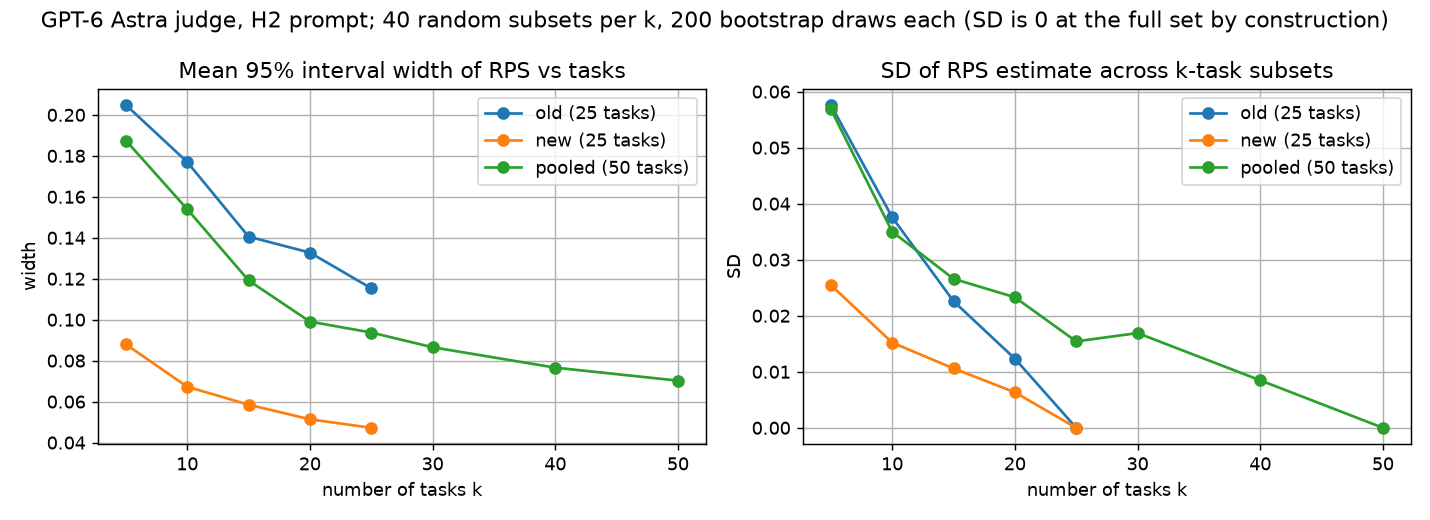
\includegraphics[width=0.85\textwidth]{figures/learning_curve_exp25.png}
\caption{Interval width and spread of the RPS estimate against the number of tasks $k$ (GPT-6 Astra, H2 prompt; 40 random task subsets per $k$, 200 bootstrap draws each). The spread is zero at the full set by construction. The width keeps falling past 25 tasks but slowly after about 30.}
\label{fig:lc}
\end{figure*}

\begin{figure*}[t]
\centering
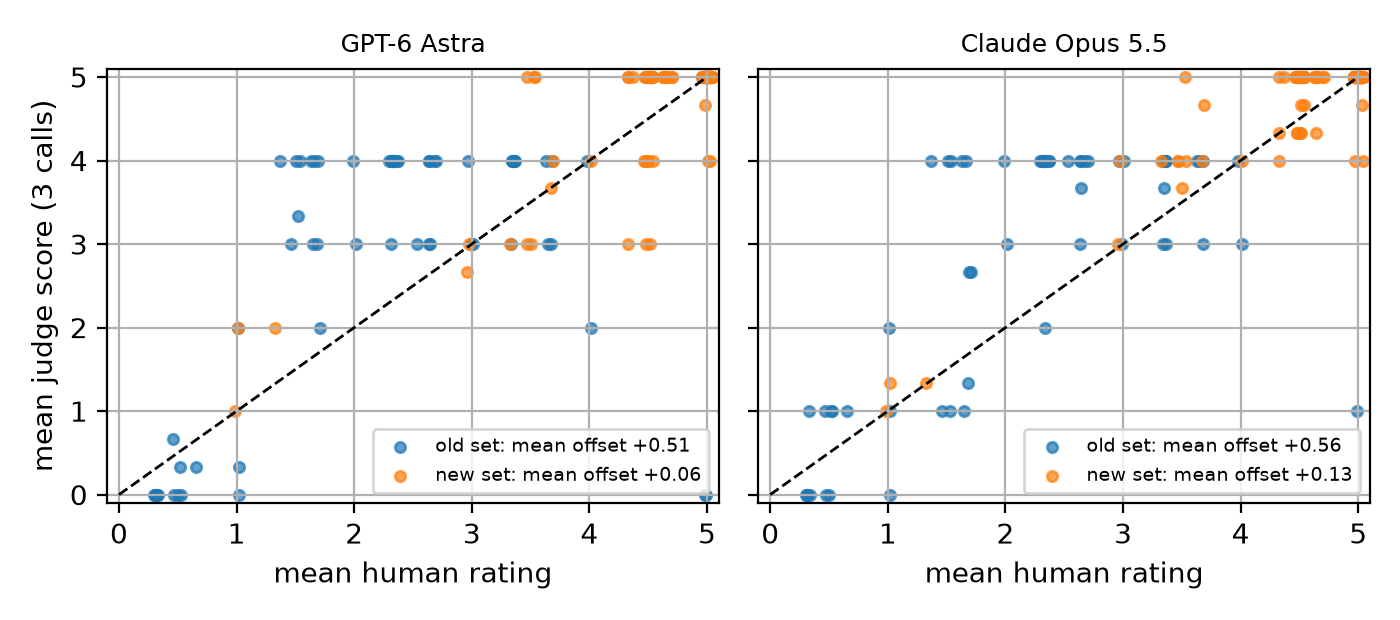
\includegraphics[width=0.8\textwidth]{figures/scatter_judge_vs_human.png}
\caption{Mean judge score (three calls, H2 prompt) against mean human rating for each of the 75 old and 100 new artifacts; dashed line is equality. The mean offset (judge minus human) is $+0.51$ and $+0.56$ on the old set but $+0.06$ and $+0.13$ on the new set, where human ratings are mostly 5s. Points are jittered by up to $0.04$ in $x$.}
\label{fig:scatter}
\end{figure*}

\paragraph{But the judge is not better.}
The pooled rows look like a large gain over the constant ($0.120$ and $0.101$ against $0.164$), but that constant mixes an old set with mean rating $2.63$ of $5$ and a new set that is mostly 5s (mean $4.57$).
Against the set-aware constant ($0.118$) the differences are $+0.002$ $[-0.030,+0.036]$ for Astra and $-0.018$ $[-0.048,+0.013]$ for Opus: neither is clearly better (both intervals contain $0$).
On the old set alone neither judge beats the constant (Astra $+0.025$, Opus $-0.003$, both intervals contain $0$).
On the new set Opus is clearly better ($-0.029$, $[-0.050,-0.009]$), Astra borderline ($-0.015$, $[-0.034,+0.002]$), against a constant that is nearly ``all 5s''.
Both judges overscore the old set by about half a point ($+0.51$ Astra, $+0.56$ Opus on the $0$ to $5$ scale, intervals above $0$; \cref{fig:scatter}), and pooling only measures that bias more tightly.
The raw pooled Spearman ($0.79$, $0.86$) is partly the difference between the sets; with ranks taken inside each set it is $0.62$ $[0.42,0.77]$ and $0.71$ $[0.56,0.81]$.

\paragraph{Human ceiling.}
Split-half Pearson between random halves of the raters is $0.83$ on the old set and $0.78$ on the new set (Spearman--Brown reliability $0.90$ and $0.88$).
On the new set the Spearman is only $0.48$ because $73\%$ of ratings are 5s, so rank correlation is a weak instrument there.
The better of the two judges scored on both sets (Opus, old-set Pearson $0.78$) sits well below the correlation ceiling ($0.95$); on the new set Opus ($0.90$) is close to its ceiling ($0.94$).

\subsection{An earlier judge panel on corrected labels}
\label{sec:cert}
An earlier panel of judges reported judge--human Spearman of $0.833$ (gpt-5.3-codex), $0.905$ (claude-opus-4-7) and $0.738$ (Qwen3-Coder) against one annotator's labels.
Those labels have Spearman $-0.04$ with the corrected VeriBench ratings on the same 59 artifacts.
\Cref{tab:cert} re-scores the saved judge outputs against the corrected labels of the corrected-label set (59 artifacts, 20 tasks, 4.5 ratings each).
No judge call was new.
None of the three headline series beats the constant (raw RPS $0.217$ to $0.271$ against $0.174$) and their point-estimate correlations are negative (the interval excludes $0$ only for Qwen3-Coder).
After leave-one-task-out calibration, the CE-fitted forecast has mean RPS $0.1725$ against $0.1737$ for the constant over the 24 series, and none of the 24 is significantly better; the Pearson-fitted forecast has the same mean ($0.1724$).
CE-fitting has lower RPS than Pearson-fitting in $13$ of $24$ series and lower CE in $15$, but lower TVD in none, and the mean RPS difference is $0.0001$ in favor of Pearson-fitting; no cell is significantly separated, so this is not a result.
The earlier direction of cross-entropy over correlation~\citep{anon2026corrce} therefore does not show up here, most likely because these judges carry almost no signal on the corrected labels and every fit collapses to the marginal.
A caveat covers the whole section: for only 7 of the 24 scored tasks is the reference file the judge saw the one the raters saw, so part of the negative numbers may come from that mismatch (untested).

\begin{table*}[t]
\caption{Headline judge series (prompt P8\_STRICT\_B) against the corrected labels, and the constant forecast (training marginal, leave-one-task-out). Task-cluster bootstrap 95\% intervals ($2{,}000$ draws). RPS, CE and TVD first.}
\label{tab:cert}
\centering\small
\begin{tabular}{lccccc}
\toprule
Series & RPS [95\%] & CE [95\%] & TVD [95\%] & Spearman [95\%] & Pearson [95\%]\\
\midrule
gpt-5.3-codex & 0.244 [0.206, 0.288] & 2.26 [2.16, 2.36] & 0.671 [0.618, 0.724] & $-$0.24 [$-$0.60, $+$0.20] & $-$0.10 [$-$0.47, $+$0.28]\\
claude-opus-4-7 & 0.271 [0.229, 0.319] & 2.30 [2.18, 2.41] & 0.689 [0.626, 0.751] & $-$0.21 [$-$0.51, $+$0.11] & $-$0.24 [$-$0.51, $+$0.07]\\
Qwen3-Coder-30B-A3B-Instruct & 0.217 [0.191, 0.248] & 2.11 [2.00, 2.22] & 0.618 [0.561, 0.678] & $-$0.35 [$-$0.59, $-$0.06] & $-$0.37 [$-$0.61, $-$0.05]\\
Constant forecast & \textbf{0.174} [0.152, 0.197] & \textbf{1.77} [1.69, 1.87] & \textbf{0.486} [0.435, 0.536] & n/a & n/a\\
\bottomrule
\end{tabular}
\end{table*}

\subsection{Building a judge that works}
\label{sec:exp27}
The results so far say that the judges we have do not beat the constant.
We therefore pre-registered, and time-stamped before any judge call or metric on the splits, an experiment to build one on the pooled old and new ratings.
\emph{Splits} are by task: old $10/5/10$ (the earlier split), new $10/5/10$ drawn with a fixed seed, so the pooled test set has 20 tasks (old 30 and new 40 artifacts).
\emph{Candidates} give a distribution over the six ratings fitted by cross-entropy on train tasks: an ordinal cumulative-logit calibration of judge-score features (GPT-6 Astra and Claude Opus 5.5 mean scores, their gap, an edit-distance similarity, and the features of a new prompt variant with train-only demonstrations, a base rate and a verbalized score distribution), optionally mixed with the train constant.
A set indicator is allowed only as a sensitivity analysis.
Selection is by lowest pooled validation RPS, then refit on train and validation and scored once on test.
\emph{``Works''} means: against both the set-aware constant and the earlier H2 judge, the paired test RPS interval lies entirely below $0$, and CE and TVD point estimates are also lower than the constant's.
``Promising, not shown'' means all three point estimates are lower but the RPS interval includes $0$; anything else is ``not found''.
\TODO{11-24-2026: results of this experiment (selected configuration, test RPS, CE, TVD with intervals, verdict against the three-level rule, per-set results); second pass after it reports. The preregistration guess is about 25\% that ``works'' is met.}
